\documentclass[11pt,a4paper]{article}

\usepackage[margin=2.4cm]{geometry}
\usepackage{amsmath,amssymb}
\usepackage{booktabs}
\usepackage{graphicx}
\usepackage{xcolor}
\usepackage{enumitem}
\usepackage{caption}
\usepackage{multirow}
\usepackage{array}
\usepackage{tikz}
\usetikzlibrary{positioning,arrows.meta,fit,backgrounds}
\usepackage[colorlinks=true,linkcolor=blue!60!black,citecolor=blue!60!black,urlcolor=blue!60!black]{hyperref}

\graphicspath{{swing_leg/fig/}}
\captionsetup{font=small,labelfont=bf,skip=4pt}
\setlist{itemsep=2pt,topsep=3pt}
\setlength{\emergencystretch}{3em}

\newcommand{\Jmat}{\mathbf{J}}
\newcommand{\Jbar}{\bar{\mathbf{J}}}
\newcommand{\Mmat}{\mathbf{M}}
\newcommand{\Kp}{\mathbf{K}_p}
\newcommand{\Kd}{\mathbf{K}_d}
\newcommand{\vp}{\mathbf{p}}
\newcommand{\vv}{\mathbf{v}}
\newcommand{\va}{\mathbf{a}}
\newcommand{\vq}{\mathbf{q}}
\newcommand{\vtau}{\boldsymbol{\tau}}
\newcommand{\ez}{\mathbf{e}_z}
\newcommand{\Nm}{\,N\,m}
\newcommand{\Nms}{\,N\,m/s}
\definecolor{bad}{HTML}{B03030}
\definecolor{good}{HTML}{1E7A4F}

\title{\textbf{DOG6 Swing-Leg Control}\\[0.3em]
\large The Control Law, and How to Carry It from Simulation onto the Robot}
\author{Eshou}
\date{1 October 2026}

\begin{document}
\maketitle

% ===========================================================================
\section*{Summary}

\begin{enumerate}[leftmargin=1.5em]
\item \textbf{The law.} A swinging foot follows a vertical bump in the
\emph{trunk} frame. The bump starts and ends at the foot position latched at
liftoff, and its height profile is two quintic halves. The joint torque has
two parts. The feedforward is leg gravity plus an optional inertial term
$\Mmat_0\ddot\vq_{ref}$, off by default. The Cartesian part is an impedance
on the foot. This is the simulator's swing law
(\S\ref{sec:law}) with three changes: no foot placement, a constant
joint-space inertia in place of the operational-space one, and no Coriolis
term.

\item \textbf{The feedforward makes the motion; the PD only corrects it.}
At the foot the swing PD is a 1\,Hz spring on a 4\,kg rotor-dominated mass. A
100--160\,ms swing is far faster than that. With the PD alone the foot reaches
55--60\,\% of the apex, and reaches it late.

\item \textbf{The slew limiter is the main gap between simulation and
hardware.} The simulator has none. On the robot every joint torque is
rate-limited to $S = 60$\Nms. In a one-leg model of the hardware chain, the
delay and the filtered velocity together cost 1--2\,mm of tracking. The slew
makes the apex late ($s = 0.66$--$0.82$ instead of $0.5$) and leaves the foot
10--20\,mm in the air when the clock hands it the load.

\item \textbf{Budget rule.} The arc's feedforward torque rate peaks at
$D \approx \kappa H/T^3$, with $\kappa \approx 70$\,N\,s$^2$ for both the
nominal and fold postures. The foot tracks once $S \ge \tfrac12 D$, that is
$H \le 2ST^3/\kappa$. Every swing flown so far needs 2.9 to 11.7 times the
60\Nms{} it gets (Table~\ref{tab:budget}).

\item \textbf{Applying it on the robot} (\S\ref{sec:method}) takes six steps.
First, put the slew into the simulator. Then identify the leg inertia on the
bench, and size $(T, H, S)$ to the budget, either with a longer swing or with
a phase-scheduled slew on the swinging joints. Keep the feedforward on. Drop
the hold-layer damper on swinging legs, which is done since 2026-10-01.
Finally, check that the foot is actually down before loading it.
\end{enumerate}

% ===========================================================================
\section{Scope and notation}

This note covers the swing phase of the in-place trot. The stance-side
balance law, the allocator and the gait clock appear only where they touch a
swinging leg.

\begin{tabbing}
\hspace{3.0cm}\=\kill
$\vq_i, \dot\vq_i$ \> leg $i$ joints (abd, pitch, knee) and rates \\
$\vp_i = \mathrm{FK}(\vq_i)$ \> foot position, trunk frame \\
$\Jmat_i$ \> foot Jacobian, trunk frame, $3\times3$ \\
$\Jbar_i$ \> its pitch and knee columns, $3\times2$; $\Jbar^+ = (\Jbar^\top\Jbar)^{-1}\Jbar^\top$ \\
$\Mmat(\vq)$, $\Mmat_0$ \> leg joint-space inertia, and its constant value at the lift pose \\
$T_g$, $d$, $T$ \> gait period, duty, swing duration $T = (1-d)\,T_g$ \\
$s = (t - t_{lo})/T$ \> swing progress, $0$ at liftoff, $1$ at the clock's touchdown \\
$H$ \> swing apex above the liftoff point \\
$S$ \> torque slew limit, N\,m/s, per joint \\
$\hat\tau$, $D$ \> peak feedforward torque, and peak feedforward torque \emph{rate}, along one arc
\end{tabbing}

All numbers in this note are for the front-left leg at the nominal lift pose
(trunk bottom 145\,mm) unless stated otherwise. The fold pose was checked
where it matters and gives the same $\kappa$ to within 2\,\%.

% ===========================================================================
\section{The control law}
\label{sec:law}

\subsection{The reference: a bump in the trunk frame, latched at liftoff}

On the first swinging sweep the measured foot position is latched,
$\vp_0 = \vp_i(t_{lo})$. The reference is a pure vertical bump on that point:
\begin{equation}
\vp_{ref}(s) = \vp_0 + z(s)\,\ez, \qquad
z(s) = \begin{cases} H\,\sigma(2s) & s \le \tfrac12 \\[2pt]
                     H\,\sigma(2-2s) & s > \tfrac12 \end{cases},
\qquad \sigma(u) = 10u^3 - 15u^4 + 6u^5 .
\label{eq:arc}
\end{equation}
$\vv_{ref} = \dot z\,\ez$ and $\va_{ref} = \ddot z\,\ez$ follow analytically.
The quintic $\sigma$ has zero first and second derivatives at both ends, so
velocity \emph{and} acceleration are zero at liftoff, at the apex and at
touchdown. Its peaks (Appendix~\ref{app:quintic}) are
\begin{equation}
\hat v = \frac{15}{4}\frac{H}{T}, \qquad
\hat a = \frac{40}{\sqrt3}\frac{H}{T^2} \approx 23.1\,\frac{H}{T^2}, \qquad
\hat{\jmath} = 480\,\frac{H}{T^3}.
\label{eq:peaks}
\end{equation}
For example, 20\,mm in 160\,ms gives 0.47\,m/s, 18\,m/s$^2$ and
2300\,m/s$^3$. The last number is the one the slew limiter sees
(\S\ref{sec:budget}).

Three design decisions are built into~\eqref{eq:arc}:
\begin{itemize}[leftmargin=1.3em]
\item \textbf{No placement.} Start and end are the same point, so the arc has
no horizontal component. It needs no velocity estimate, no world position and
no rotation; DOG6 had none of the three when this was chosen. The cost is
that the foot cannot be held still in the \emph{world}: a trunk that moves
during the swing carries the foot with it.
\item \textbf{Latched, not commanded.} The arc starts where the foot
\emph{is}, not at a nominal resting site. The joint-hold layer pinned the
stance at the angles latched on reaching HOLD (its spring is out since
2026-10-02; the damper stays). A resting site that differs
from where the feet stand is therefore a step every swing, and two fixed
points that disagree walk the trunk. A single latched point cannot walk.
\item \textbf{Trunk frame.} No $\mathbf{R}$ appears anywhere in the swing
law, so nothing in it can be wrong about attitude.
\end{itemize}

\subsection{The torque law on the robot}

The swing torque on leg $i$ has two parts. The \emph{feedforward} depends
only on the reference and the leg model, and is computed open loop. The
\emph{Cartesian} part depends on the measured foot, and closes the loop:
\begin{equation}
\boxed{\;\vtau_i = \vtau_i^{ff} + \vtau_i^{cart}\;}
\label{eq:law}
\end{equation}

\paragraph{Part 1: the feedforward.}
\begin{equation}
\vtau_i^{ff} = \underbrace{\mathbf{g}_i(\vq_i)}_{\text{leg weight, always on}}
+ \underbrace{\Mmat_0\,\ddot\vq_{ref}}_{\text{leg inertia, switchable}}
\label{eq:ff}
\end{equation}
The joint-space reference comes through the pitch and knee columns, with
abduction held:
\begin{equation}
\dot\vq_{ref} = \begin{bmatrix}0\\ \Jbar_i^+\vv_{ref}\end{bmatrix}, \qquad
\ddot\vq_{ref} = \begin{bmatrix}0\\ \Jbar_i^+\!\left(\va_{ref} - \dot\Jmat_i\dot\vq_{ref}\right)\end{bmatrix}.
\label{eq:qref}
\end{equation}
\begin{itemize}[leftmargin=1.3em]
\item $\mathbf{g}_i$ comes through the stance path. The allocator gives a
swinging foot zero force, and the stance torque adds every leg's own weight,
so the swing leg receives exactly its gravity.
\item $\Mmat_0\ddot\vq_{ref}$ is the torque the arc's acceleration needs. On
the robot it is \textbf{exactly what \texttt{-{}-swing-ff} switches}, and
nothing else. The flag does not touch $\mathbf{g}_i$ or Part~2. It is
\textbf{off by default}. With it off, $\vtau_i^{ff} = \mathbf{g}_i$: the
feedforward holds the leg up and does nothing to move it,
and~\eqref{eq:qref} is not needed at all. With it on, this term's share of
the torque is logged on its own (\texttt{tau\_ff}).
\item $\dot\Jmat\dot\vq_{ref}$ is evaluated at the \emph{reference} rate, by
one extra Jacobian at $\vq + \epsilon\dot\vq_{ref}$. Without it the chain's
own curvature pushes the foot off the vertical line: 4.3\,mm of $x$ at
touchdown, against 0.8\,mm with it.
\end{itemize}

\paragraph{Part 2: the Cartesian impedance.}
\begin{equation}
\vtau_i^{cart} = \Jmat_i^\top\!\left[\Kp(\vp_{ref}-\vp_i) + \Kd(\vv_{ref}-\Jmat_i\dot\vq_i)\right]
\label{eq:cart}
\end{equation}
\begin{itemize}[leftmargin=1.3em]
\item $\Kp = \mathrm{diag}(140, 140, 180)$\,N/m and
$\Kd = \mathrm{diag}(8, 8, 15)$\,N\,s/m are the DOG5 defaults. The bench
settled on $\Kd = \mathrm{diag}(20,20,40)$ with the feedforward off, and that
is the value used in \S\ref{sec:oneleg}.
\item This is the only part that reads the measured foot. It is not purely
feedback, however: $\Kd\vv_{ref}$ is a velocity feedforward hidden inside
the damper. With the inertial term off it is the \emph{only} thing that
anticipates the motion (\S\ref{sec:gains}).
\end{itemize}

\paragraph{Nothing else, since 2026-10-01.} The trot's joint-hold layer
adds $K_p(\vq_{hold}-\vq) - K_h\dot\vq$ to every \emph{planted} leg, with
$K_h = 0.2$\,N\,m\,s/rad; $K_p$ has been $0$ since 2026-10-02, on request,
so a planted leg gets the damper alone. Until 2026-10-01 a swinging leg kept the damper
$-K_h\dot\vq_i$: its spring target followed the leg, but the damper stayed,
and it was \emph{absolute}. The MIT method has no such term, and the
simulator damps stance legs only. The damper is now dropped on swinging legs,
so what reaches the gate for a swinging leg is exactly
$\vtau_i^{ff} + \vtau_i^{cart}$, in the trot as on the bench. See
\S\ref{sec:method}, step~\ref{step:damper}.

\paragraph{Which hardware flag sets which term.} Table~\ref{tab:flags} maps
each term to the flags that switch or set it. The trot entry points and the
swing bench share these flags and their defaults.

\begin{table}[htbp]
\centering
\caption{The terms of the swing torque and the flags that control them on the
robot.}
\label{tab:flags}
\small
\begin{tabular}{@{}lll>{\raggedright\arraybackslash}p{6.2cm}@{}}
\toprule
term & part & default & flag \\
\midrule
$\mathbf{g}_i(\vq_i)$, leg weight & 1, ff & on & none: always on \\
$\Mmat_0\ddot\vq_{ref}$, leg inertia & 1, ff & \textbf{off} & \texttt{-{}-swing-ff} turns it on;
  \texttt{-{}-ff-armature} sets the armature inside $\Mmat_0$ (default 0.0085\,kg\,m$^2$, DOG5's) \\
$\Jmat^\top[\Kp\mathbf{e}_p + \Kd\mathbf{e}_v]$ & 2, cart & on & always on;
  \texttt{-{}-kp-swing}, \texttt{-{}-kd-swing} set the gains (140/140/180, 8/8/15);
  \texttt{-{}-swing joint} replaces it with a joint PD \\
$-K_h\dot\vq_i$, hold damper & neither & \textbf{removed} & none on swinging legs
  since 2026-10-01; \texttt{-{}-kd-joint} (0.2) now sets stance legs only \\
\midrule
the arc $\vp_{ref}, \vv_{ref}, \va_{ref}$ & feeds both & --- & \texttt{-{}-swing-height} sets $H$;
  \texttt{-{}-period} sets $T = (1-d)\,T_g$ \\
\bottomrule
\end{tabular}
\end{table}

\subsection{Relation to the simulator's swing law}

The simulator runs the convex-MPC swing law: Raibert placement plus an
operational-space impedance. It splits into the same two parts:
\begin{align}
\vp_{td} &= \vp_{hip} + \tfrac12\,\vv_{CoM}\,T_{st} \qquad \text{(world frame)} \label{eq:raibert}\\
\vtau_i &= \underbrace{\Jmat^\top\boldsymbol{\Lambda}\left(\va_{ref} - \dot\Jmat\dot\vq\right)
 + \mathbf{C}\dot\vq + \mathbf{G}}_{\vtau^{ff}}
 \;+\; \underbrace{\Jmat^\top\!\left[\Kp\mathbf{e}_p + \Kd\mathbf{e}_v\right]}_{\vtau^{cart}},
 \qquad \boldsymbol\Lambda = (\Jmat\Mmat^{-1}\Jmat^\top)^{-1}. \label{eq:cmpc}
\end{align}
The Cartesian parts differ only in gains and frame. The feedforward parts
differ in what they model. For a square, invertible $\Jmat$,
$\Jmat^\top\boldsymbol\Lambda = \Mmat\Jmat^{-1}$, so the operational-space
term is \emph{identical} to $\Mmat\,\ddot\vq_{ref}$. The robot's inertial
term in~\eqref{eq:ff} is the same thing with three approximations:
\begin{enumerate}[leftmargin=1.5em]
\item $\Mmat(\vq) \to \Mmat_0$. The reflected rotor is 61\,\% and 96\,\% of
the pitch and knee diagonal. No off-diagonal entry exceeds 0.0006\,kg\,m$^2$,
and $\Mmat$ barely moves along an in-place $z$ arc.
\item $\Jmat^{-1} \to \Jbar^+$, with abduction held, because the arc has no
$y$.
\item $\mathbf{C}\dot\vq$ is dropped. It is 0.01\Nm, because the rotor that
dominates $\Mmat$ has no velocity term.
\end{enumerate}
The gain is cost: 57\,$\mu$s per leg, against 2.2\,ms per leg for
$\boldsymbol\Lambda$ and the RNEA on the Pi. Table~\ref{tab:laws} lists
everything that differs.

\begin{table}[htbp]
\centering
\caption{The two swing laws side by side.}
\label{tab:laws}
\small
\begin{tabular}{@{}lll@{}}
\toprule
 & simulator (convex MPC) & robot \\
\midrule
reference frame & world, converted to body each step & trunk, no rotation used \\
foot placement & Raibert, eq.~\eqref{eq:raibert} & none; lands where it lifted \\
arc start & foot at liftoff & foot at liftoff (latched) \\
arc shape & quintic halves, 30\,mm, 250\,ms & quintic halves, 20--40\,mm, 100--160\,ms \\
feedforward & $\Jmat^\top\boldsymbol\Lambda(\va - \dot\Jmat\dot\vq) + \mathbf{C}\dot\vq + \mathbf{G}$ & $\Mmat_0\ddot\vq_{ref} + \mathbf{g}$ (inertial term optional) \\
impedance & $500/20$ isotropic & $140/140/180$, $\Kd$ 8/8/15 or 20/20/40 \\
extra damping & none & none since 2026-10-01 (was $-0.2\,\dot\vq$) \\
state used & true $\vq, \dot\vq$, world pose & encoders, filtered $\dot\vq$ \\
torque path & clamp 8\Nm & ramp, cap 9\Nm, limit block, \textbf{slew 60\Nms} \\
\bottomrule
\end{tabular}
\end{table}

\subsection{What the gains can and cannot do}
\label{sec:gains}

Seen from the foot, the leg is strongly anisotropic. At the lift pose the
apparent mass is $m_z = 4.07$\,kg vertically and $m_x = 0.39$\,kg fore-aft,
almost all of it reflected rotor. The vertical PD is then
\[
\omega_{n,z} = \sqrt{K_{p,z}/m_z} = 6.7\,\text{rad/s}\;(1.1\,\text{Hz}), \quad
\zeta = \frac{K_{d,z}}{2\sqrt{K_{p,z} m_z}} = 0.28\;(K_{d,z}{=}15),\ 0.74\;(K_{d,z}{=}40).
\]
A 160\,ms swing has its content near 6\,Hz, five times above that natural
frequency. The PD cannot \emph{generate} the motion; it can only correct
around a motion produced by something else. On the simulator's own chain, the
PD alone reaches 54--59\,\% of the apex at $s \approx 0.76$
(Table~\ref{tab:chain}). The two ways to supply the motion are the inertial
feedforward, and the $\Kd\vv_{ref}$ part of the damper. The latter is a
velocity feedforward that lags the needed torque by a quarter cycle and has
no inertia in it.

Stiffening $K_{p,z}$ is not a substitute. Without $\boldsymbol\Lambda$, a $z$
force at the foot accelerates the foot along $\Mmat^{-1}\Jmat^\top\ez$, which
has an $x$ component. Raising $K_{p,z}$ from 180 to 800 took the $x$ drift
from 2 to 10\,mm. This is why the simulator can use one isotropic gain and the
robot cannot.

% ===========================================================================
\section{Between the law and the joint: what the robot adds}
\label{sec:chain}

\begin{figure}[htbp]
\centering
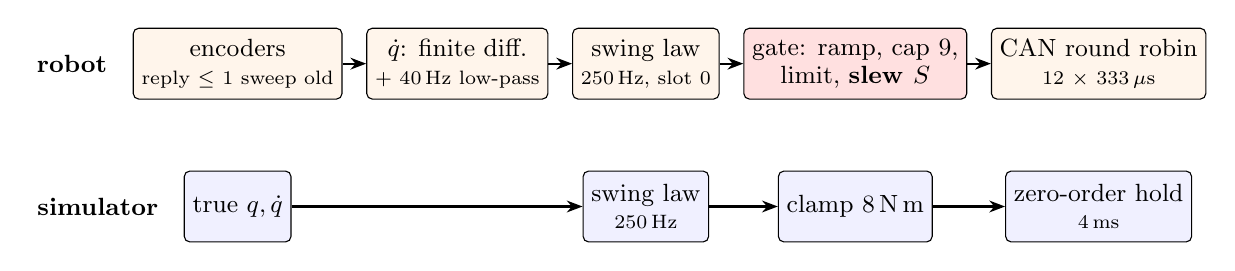
\begin{tikzpicture}[
  font=\small, node distance=3mm,
  blk/.style={draw, rounded corners=2pt, minimum height=9mm, align=center, inner sep=3pt},
  hw/.style={blk, fill=orange!8},
  sm/.style={blk, fill=blue!6},
  arr/.style={-{Stealth[length=2mm]}, thick}]
\node[hw] (enc) {encoders\\[-1pt]\scriptsize reply $\le$ 1 sweep old};
\node[hw, right=of enc] (vel) {$\dot q$: finite diff.\\[-1pt]\scriptsize + 40\,Hz low-pass};
\node[hw, right=of vel] (law) {swing law\\[-1pt]\scriptsize 250\,Hz, slot 0};
\node[hw, right=of law, fill=red!12] (gate) {gate: ramp, cap 9,\\[-1pt]limit, \textbf{slew $S$}};
\node[hw, right=of gate] (can) {CAN round robin\\[-1pt]\scriptsize 12 $\times$ 333\,$\mu$s};
\draw[arr] (enc) -- (vel); \draw[arr] (vel) -- (law); \draw[arr] (law) -- (gate);
\draw[arr] (gate) -- (can);
\node[sm, below=9mm of enc] (st) {true $q, \dot q$};
\node[sm] (law2) at (law |- st) {swing law\\[-1pt]\scriptsize 250\,Hz};
\node[sm] (clamp) at (gate |- st) {clamp 8\Nm};
\node[sm] (zoh) at (can |- st) {zero-order hold\\[-1pt]\scriptsize 4\,ms};
\draw[arr] (st) -- (law2); \draw[arr] (law2) -- (clamp); \draw[arr] (clamp) -- (zoh);
\node[left=2mm of enc, font=\small\bfseries, anchor=east] {robot};
\node[left=2mm of st, font=\small\bfseries, anchor=east] {simulator};
\end{tikzpicture}
\caption{The actuation chain on the robot (top) and in the simulator
(bottom). The swing law is the same box in both. Everything orange is
hardware the simulator does not model, and the red box is the one that
matters.}
\label{fig:chain}
\end{figure}

Figure~\ref{fig:chain} and Table~\ref{tab:gap} list what the robot puts
between the law and the joint. The question is which items matter for a
swing.

\begin{table}[htbp]
\centering
\caption{The simulation-to-hardware gap, item by item, for a swinging leg.
``Effect'' is measured in the one-leg model of \S\ref{sec:oneleg}.}
\label{tab:gap}
\small
\begin{tabular}{@{}p{2.5cm}p{3.1cm}p{5.2cm}p{3.6cm}@{}}
\toprule
item & simulator & robot & effect on a swing \\
\midrule
torque rate & unlimited & $|\dot\tau| \le 60$\Nms{} per joint (the gate's slew, DOG5's trot value) & \textcolor{bad}{\textbf{dominant}}: late apex, late touchdown, hard landing \\
torque cap & 8\Nm & 9\Nm, ramped from 0 over 1\,s at arming & binds only for $T \lesssim 100$\,ms \\
timing & 4\,ms hold, fresh state & law at slot 0; motor $j$ commanded $j \times 0.33$\,ms later; replies up to one sweep old; one motor in twelve at 8\,ms each status sweep & 1--2\,mm rms, together with the filter \\
joint velocity & exact & encoder difference, 40\,Hz low-pass ($\approx$4\,ms lag) & (with timing) \\
leg inertia & the model \emph{is} the plant & armature inherited from DOG5, not measured; 61--96\,\% of $\Mmat$ & feedforward gain error: 1.6$\times$ apex if the rotor is half the model's \\
state & world pose and velocity & no world pose, no contact sensing & no placement; contact is a timetable \\
compute & unbounded & law must fit a 333\,$\mu$s slot (already over) & $\Mmat_0$ instead of $\boldsymbol\Lambda$ \\
extra torque & none & $-0.2\,\dot\vq$ hold damper on the swinging leg; removed 2026-10-01 & halved the apex on a feasible arc \\
\bottomrule
\end{tabular}
\end{table}

\subsection{The slew limiter as a dynamic element}

The gate passes each joint's request through a rate limiter, sweep by sweep:
\begin{equation}
\tau_k = \tau_{k-1} + \mathrm{sat}_{S\Delta t}\!\left(\tau_k^{req} - \tau_{k-1}\right), \qquad \Delta t = 4\,\text{ms}.
\label{eq:slew}
\end{equation}
Three properties follow.
\begin{enumerate}[leftmargin=1.5em]
\item It passes a request unchanged if and only if $|\dot\tau^{req}| \le S$
everywhere. Below that it is transparent; above it, it is a different
actuator.
\item For a sinusoidal request $A\sin\omega t$ it saturates once
$A\omega > S$. The output then becomes a triangle wave of amplitude at most
$\pi S/(2\omega)$, and its lag grows toward a quarter period. Unlike a
torque cap, it costs \emph{phase} as well as amplitude.
\item \textbf{Inside a feedback loop it winds up.} While the output ramps
behind the request, the tracking error grows and the PD keeps adding to the
request. When the arc reverses, at the apex and again on the braking half,
the limiter is still ramping the old way. The result is a late apex, an
overshoot, and a braking torque that arrives late, so the foot reaches the
ground with descent speed. This is integrator windup with the rate limiter as
the saturating element.
\end{enumerate}
The simulator has none of this, so any swing timing or gain tuned in the
simulator was tuned against a different actuator.

\subsection{The swing's torque-rate bill}
\label{sec:budget}

Along the arc, the feedforward is roughly
$\vtau_{ff} \approx \Mmat_0\Jbar^+\ddot z\,\ez$. Its rate is therefore driven
by the arc's jerk, and~\eqref{eq:peaks} puts the jerk peaks at liftoff, at
the apex and at touchdown:
\begin{equation}
D \equiv \max_t\,|\dot\tau_{ff}| \approx \kappa\,\frac{H}{T^3}, \qquad
\hat\tau \approx 3.3\,\frac{H}{T^2}, \qquad
\frac{D}{\hat\tau} \approx \frac{21}{T}.
\label{eq:budget}
\end{equation}
$\kappa \approx 70$\,N\,s$^2$ for the knee at the nominal lift pose, and 71 at
the fold lift pose, with the inherited armature. It is computed along the arc
through the IK and checked at four $(T,H)$ pairs. Because $\kappa$ is
proportional to the joint inertia, it must be recomputed once the armature is
measured.

Table~\ref{tab:budget} prices every swing flown so far. Two points stand out.
First, the cube in $T$: halving the swing costs eight times the slew.
Second, the ``slew to rise'' rule in the run banner, $4\hat\tau/T$, is five
times below $D$. The banner's empirical ``$\times3$ to land softly''
($12\hat\tau/T$) is close to the practical requirement $\tfrac12 D$ found in
\S\ref{sec:oneleg}.

\begin{table}[htbp]
\centering
\caption{The slew each swing asks for (knee, quintic arc, inherited armature).
$\tfrac12 D$ is the practical requirement from \S\ref{sec:oneleg}; the last
column is that requirement over the 60\Nms{} the gate allows.}
\label{tab:budget}
\small
\begin{tabular}{@{}lrrrrrrr@{}}
\toprule
setting & $T$ (ms) & $H$ (mm) & $\hat\tau$ (N\,m) & $4\hat\tau/T$ & $D$ (N\,m/s) & $\tfrac12 D$ & $\tfrac12 D / 60$ \\
\midrule
bench & 140 & 20 & 3.33 & 95 & 511 & 256 & \textcolor{bad}{4.3} \\
trot, 0.8\,s & 160 & 40 & 4.92 & 123 & 685 & 343 & \textcolor{bad}{5.7} \\
trot, 0.8\,s & 160 & 20 & 2.55 & 64 & 342 & 171 & \textcolor{bad}{2.9} \\
fold trot, 0.5\,s & 100 & 20 & 6.53 & 261 & 1403 & 702 & \textcolor{bad}{11.7} \\
DOG5, 1.2\,s & 240 & 40 & 2.18 & 36 & 203 & 102 & \textcolor{bad}{1.7} \\
\midrule
simulator (no slew) & 250 & 30 & 1.54 & 25 & 135 & 68 & --- \\
1.2\,s, duty 0.8 & 240 & 20 & 1.13 & 19 & 101 & 51 & \textcolor{good}{0.85} \\
1.0\,s, duty 0.7 & 300 & 20 & 0.73 & 10 & 52 & 26 & \textcolor{good}{0.43} \\
\bottomrule
\end{tabular}
\end{table}

% ===========================================================================
\section{One-leg check: the simulator's chain against the robot's}
\label{sec:oneleg}

\paragraph{Model.} One leg hangs from a pinned trunk, integrated at 4\,kHz on
its RNEA dynamics with the armature on the diagonal. There is no floor. The
swing law is~\eqref{eq:law} with $\Kd = 20/20/40$. Two chains are compared:
\begin{itemize}[leftmargin=1.3em]
\item \emph{sim}: this sweep's $\vq$, the true $\dot\vq$, and the torque held
for 4\,ms.
\item \emph{hw}: last sweep's $\vq$ and a finite-differenced $\dot\vq$ through
the 40\,Hz low-pass, then the 9\Nm{} cap and the slew~\eqref{eq:slew}.
\end{itemize}
``$z_{td}$'' is how high the foot still is when the clock declares
touchdown. On the floor, a positive value means the stance law is loading a
foot that is in the air. $v_{td}$ is the foot's vertical speed at that
moment.

\begin{table}[htbp]
\centering
\caption{One leg, 20\,mm apex. ``ff'' is the inertial feedforward. Apex is in
mm, with the progress $s$ at which it is reached; the arc's own apex is at
$s=0.5$.}
\label{tab:chain}
\small
\begin{tabular}{@{}llrrrrr@{}}
\toprule
& chain & apex (mm) @ $s$ & rms (mm) & $z_{td}$ (mm) & $v_{td}$ (m/s) & $|x|$ (mm) \\
\midrule
\multirow{6}{*}{\rotatebox{90}{\small 160\,ms}}
& sim, PD only            & 11.8 @ .76 & 8.9 & 9.2 & $-0.10$ & 2.9 \\
& sim, PD + ff            & 20.4 @ .51 & 0.5 & $-0.1$ & $-0.04$ & 0.3 \\
& hw, no slew, PD + ff    & 21.9 @ .49 & 1.1 & $-1.6$ & $-0.04$ & 0.9 \\
& hw, slew 60, PD only    & 12.4 @ .76 & 8.7 & 9.2 & $-0.12$ & 3.7 \\
& hw, slew 60, PD + ff    & \textcolor{bad}{27.1 @ .66} & 9.3 & \textcolor{bad}{9.7} & \textcolor{bad}{$-0.47$} & 5.9 \\
& hw, slew 60, PD + hold damper & 7.4 @ .66 & 8.8 & 2.7 & $-0.09$ & 3.7 \\
\midrule
\multirow{5}{*}{\rotatebox{90}{\small 100\,ms}}
& sim, PD + ff            & 20.7 @ .54 & 1.3 & 1.1 & $-0.12$ & 0.4 \\
& hw, no slew, PD + ff    & 22.3 @ .50 & 1.7 & $-0.4$ & $-0.17$ & 1.3 \\
& hw, slew 60, PD only    & 11.7 @ .94 & 10.2 & 11.6 & $-0.02$ & 6.5 \\
& hw, slew 60, PD + ff    & \textcolor{bad}{12.0 @ .82} & 9.4 & \textcolor{bad}{11.4} & $-0.08$ & 0.6 \\
& hw, slew 60, PD + hold damper & 9.1 @ .86 & 9.9 & 8.2 & $-0.11$ & 8.5 \\
\bottomrule
\end{tabular}
\end{table}

\begin{figure}[htbp]
\centering
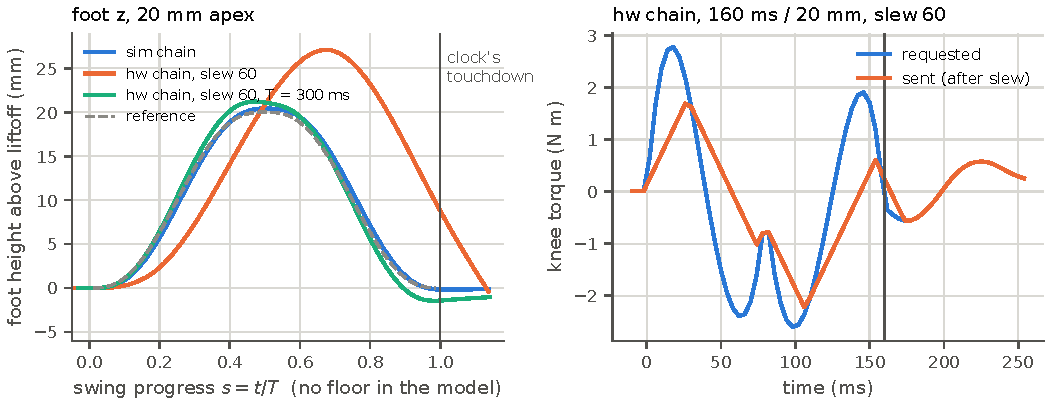
\includegraphics[width=\linewidth]{one_leg.pdf}
\caption{Left: foot height for the 0.8\,s trot's 160\,ms / 20\,mm arc. The
simulator's chain tracks the arc. The robot's chain with the 60\Nms{} slew
peaks late and high, and is still 10\,mm up at the clock's touchdown. The
same chain on a 300\,ms swing (aqua, plotted against its own $s$) tracks.
Right: the knee torque the law requests and what the slew lets through. The
request grows while the output ramps, which is the windup.}
\label{fig:oneleg}
\end{figure}

\paragraph{What the table says.}
\begin{itemize}[leftmargin=1.3em]
\item \textbf{The slew is the gap.} Take the slew out and the robot's
chain, with delay and filtered velocity, is within 1--2\,mm of the
simulator's. Put the slew in and the swing is a different motion.
\item With the slew, adding the feedforward makes the apex \emph{higher and
later}, not more accurate. The torque arrives a quarter cycle late, so it
lifts the foot during what should be the descent.
\item The 100\,ms fold swing is past the slew almost entirely: the knee
torque can rise only 1.5\Nm{} in the first quarter of the swing, against a
6.5\Nm{} request.
\end{itemize}

\paragraph{How much slew is enough.} Sweeping $S$ as a fraction of $D$
(Table~\ref{tab:threshold}) gives the same answer for every $(T,H)$ tried. The
foot tracks once $S \ge 0.4$--$0.5\,D$, and degrades quickly below $0.3\,D$.
The quintic's jerk peaks are brief, so the limiter can fall behind for a few
milliseconds and catch up. That gives the practical feasibility condition
\begin{equation}
\boxed{\;S \;\ge\; \tfrac12\,\kappa\,\frac{H}{T^3}
\quad\Longleftrightarrow\quad
H \;\le\; \frac{2\,S\,T^3}{\kappa} \approx \frac{S\,T^3}{35}\;}
\label{eq:feasible}
\end{equation}
(SI units). Design to $0.6\,D$ to leave room for the PD.
Figure~\ref{fig:budget} draws~\eqref{eq:feasible} with the flown settings on
it.

\begin{table}[htbp]
\centering
\caption{Slew as a fraction of the arc's peak torque rate $D$ (robot chain,
PD + ff). Each cell is apex progress $s$ / $z_{td}$ in mm / $v_{td}$ in m/s.}
\label{tab:threshold}
\small
\begin{tabular}{@{}lccc@{}}
\toprule
$S/D$ & 160\,ms / 20\,mm ($D$ = 342) & 100\,ms / 20\,mm ($D$ = 1403) & 240\,ms / 20\,mm ($D$ = 101) \\
\midrule
0.2 & .64 / 4.7 / $-0.47$ & .66 / 12.2 / $-0.58$ & .66 / 4.4 / $-0.38$ \\
0.3 & .59 / 0.9 / $-0.22$ & .58 / 3.0 / $-0.41$ & .58 / 0.3 / $-0.13$ \\
0.4 & .51 / $-2.1$ / $-0.07$ & .54 / $-1.2$ / $-0.24$ & .49 / $-2.4$ / $-0.02$ \\
0.5 & .49 / $-3.0$ / $-0.04$ & .50 / $-2.2$ / $-0.19$ & .48 / $-2.8$ / $\phantom{-}0.00$ \\
1.0 & .49 / $-1.6$ / $-0.04$ & .50 / $-0.4$ / $-0.17$ & .48 / $-1.6$ / $\phantom{-}0.00$ \\
\bottomrule
\end{tabular}
\end{table}

\begin{figure}[htbp]
\centering
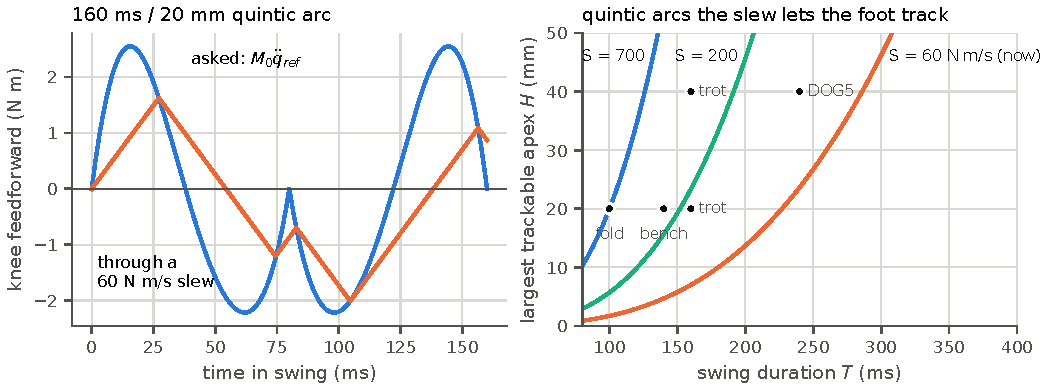
\includegraphics[width=\linewidth]{slew_budget.pdf}
\caption{Left: the knee feedforward a 160\,ms / 20\,mm arc asks for, and what
a 60\Nms{} limiter makes of it. Right: condition~\eqref{eq:feasible}, the
largest apex the foot can track for a given swing duration and slew. Points
are the settings flown so far; the 0.8\,s and 0.5\,s trots, the bench and
DOG5's clock all sit above the 60\Nms{} line.}
\label{fig:budget}
\end{figure}

\paragraph{A jerk-limited arc does not buy much.} An arc whose jerk is
bang-bang (piecewise-constant $\pm j$) needs 2.45 times less \emph{peak} rate
than the quintic for the same $(T,H)$. However, its rate is sustained, so it
needs $S \ge 0.9$--$1.0\,D$ rather than $\tfrac12 D$. The net gain is about
$1.2\times$ in apex, at 28\,\% more peak torque. It is not worth changing the
arc for.

\paragraph{Limits of the model.} The trunk is pinned and there is no floor,
so it shows the \emph{leg's} response to the chain and nothing about the
trunk. The plant is the model, so the armature is assumed right except where
stated. Only one leg and one posture were run, although $\kappa$ was checked
in the fold pose.

% ===========================================================================
\section{How to apply the law on the robot}
\label{sec:method}

The order matters: each step changes the numbers the next one is sized with.

\begin{enumerate}[leftmargin=1.6em, label=\textbf{Step \arabic*.}, ref=\arabic*]

\item \label{step:sim}\textbf{Put the actuation chain into the simulator
before tuning anything.} That means the slew~\eqref{eq:slew}, the cap and its
ramp, the one-sweep-old measurement, the finite-difference velocity with its
40\,Hz filter, and the round-robin command timing. A swing period, apex or
gain chosen in a simulator without the slew was chosen for a different
actuator. The convex-MPC simulator's 250\,ms / 30\,mm swing needs 68\Nms{} by
\eqref{eq:feasible}, more than the gate allows, and this was never visible
there.

\item \label{step:ident}\textbf{Measure the leg's inertia on the bench, with
the robot hung up.} For each swing, fit pitch and knee separately by least
squares:
\[
\tau^{meas}_j - g_j(\vq) = I_j\,\ddot q_j + b_j\,\dot q_j + c_j ,
\]
with $\tau^{meas}$ the driver's reported current times $K_t$, and $\ddot q$
from smoothed encoder data. Use the \emph{measured} torque, not the request:
the request is what the slew clipped. The knee's $\Mmat_0$ is 96\,\% rotor,
so its fit is the cleaner armature estimate. Then rebuild $\Mmat_0$ and
recompute $\kappa$.

The 1.7$\times$ apex overshoot seen on the bench does not by itself show
that the armature is wrong. In the one-leg model, with the armature right,
slew windup alone gives 1.37$\times$ on a 15\,mm / 140\,ms arc. With half
the armature and no slew, a 160\,ms / 20\,mm arc overshoots 1.6$\times$. Both
together on the 15\,mm / 140\,ms arc give 2.1$\times$, $|x| = 12$\,mm and $v_{td} = -0.7$\,m/s. That last case is close
to what the bench saw (26\,mm for 15, 15--21\,mm of $x$, $-0.3$ to
$-0.65$\,m/s). Only the regression separates the two causes.

\item \label{step:size}\textbf{Size $(T, H, S)$ to the budget}, using
\eqref{eq:feasible} at $S \ge 0.6\,D$. There are three levers, in order of
strength:
\begin{enumerate}[label=(\alph*), leftmargin=1.4em]
\item \emph{Swing duration $T = (1-d)T_g$, which enters as the cube.} At
60\Nms, DOG5's clock ($T_g = 1.2$\,s, $d = 0.8$, $T = 240$\,ms) tracks a
20\,mm arc: apex 20.8\,mm at $s = 0.48$, $z_{td} = -2.2$\,mm, $v_{td} = 0$.
$T_g = 1.0$\,s at $d = 0.7$ gives $T = 300$\,ms, which tracks 20\,mm with
margin ($\tfrac12 D = 26$\Nms) and even 30\,mm.

The duty cannot be lowered freely. The clock needs all four feet at full
weight at the middle of the four-foot window, which requires a contact ramp
$r \le (d - 0.5)/(2d)$. At $d = 0.7$ that is $r \le 0.14$, and the stance
handover then takes $r\,d\,T_g = 98$\,ms, the same as today's 0.8\,s trot. At
$T_g = 0.8$\,s and $d = 0.6$ the ramp would have to drop to 0.08, and a 38\,ms
handover is past the \emph{stance} slew. A lower duty also means longer
two-foot phases, where the trot's roll already has least to push against.
\item \emph{A phase-scheduled slew.} Give a joint $S_{sw}$ while its leg's
contact weight is zero, and the stance value of 60 otherwise. Switch the
\emph{limit}, not the torque, so the change is bumpless. The slew exists to
turn controller discontinuities into ramps. The swing request is $C^2$ by
construction: the feedforward is zero at liftoff and touchdown and
continuous between. The discontinuities the slew guards against sit at the
contact handover, which keeps 60. For the 0.8\,s trot,
$S_{sw} \approx 200$ (20\,mm) or 400 (40\,mm). The 0.5\,s fold trot would need
about 850, with a 7.5\Nm{} peak against the 9\Nm{} cap; do not fly that
swing. What a high $S_{sw}$ no longer filters is a PD kick in the air,
meaning velocity noise times $\Kd$. Keep $\Kd$ at the value the bench needed,
not higher.
\item \emph{Apex $H$, which is linear.} At 160\,ms and 60\Nms{} the
trackable apex is 7\,mm. That is the cheapest lever and the least useful one
on a real floor.
\end{enumerate}

\item \label{step:ff}\textbf{Let the feedforward make the motion, and keep
the PD small.} With a measured $\Mmat_0$ and a feasible arc, the PD error
stays around 1\,mm and its gains matter little. Leave $K_{p,z}$ alone, because
without $\boldsymbol\Lambda$ it pushes the foot into $x$. Keep $K_{d,z}$
around 30--40 ($\zeta \approx 0.6$--$0.75$). Flying $\Kd\vv_{ref}$ without
the feedforward (the bench's 20/20/40) is a usable fallback, but in the model
it reaches only 55--77\,\% of the apex depending on the armature, and always
late ($s \approx 0.75$). A height read by eye cannot show that lateness; the
log's apex timing will.

\item \label{step:damper}\textbf{No hold damper on a swinging leg (done,
2026-10-01).} The hold layer's $-K_h\dot\vq$ on a swinging leg was
$83$\,N\,s/m at the foot in $z$. That is twice the swing PD's own $K_{d,z}$,
and all of it opposed the arc. On a feasible 300\,ms / 20\,mm swing it
halved the apex (21.2 to 11.2\,mm). It is now dropped on swinging legs, as in
the MIT method and the simulator, and the trot's swing is the bench's swing.
A relative form, $-K_h(\dot\vq - \dot\vq_{ref})$, would have kept some
abduction damping, but the Cartesian $\Kd$ already gives abduction 0.22 to
0.55\,N\,m\,s/rad. On the arcs flown so far, which are past the budget, the
drag was partly masking the windup. Without it, at 0.8\,s / 20\,mm and slew
60, the PD alone lifts higher (12.4 against 7.4\,mm, still late), and with
\texttt{-{}-swing-ff} on the apex overshoots more (27.1 against 22.2\,mm at
$s = 0.66$). Step~\ref{step:size} is what fixes that.

\item \label{step:td}\textbf{Do not load a foot that is not down.} The clock
hands the load over at $s = 1$ whatever the foot is doing, and the slew makes
the foot late. The cheapest guard is kinematic: hold the stance contact ramp
at zero until the foot's trunk-frame $z$ is within a few millimetres of its
latched liftoff $z$ (or a short timeout passes). Log $z_{td}$ and $v_{td}$
for every swing.

\end{enumerate}

\paragraph{Acceptance per swing,} on the bench first and then on the floor:
slew clip on the swinging joints below 0.3\Nm{}; apex within $\pm15\,\%$ of
$H$, reached at $s \in [0.45, 0.55]$; $|z_{td}| \le 3$\,mm;
$|v_{td}| \le 0.1$\,m/s; $|x| \le 3$\,mm. The bench analysis already
reports every one of these quantities.

\begin{table}[htbp]
\centering
\caption{The design options in the one-leg model, robot chain throughout.}
\label{tab:options}
\small
\begin{tabular}{@{}lrrrrr@{}}
\toprule
option & apex (mm) @ $s$ & rms & $z_{td}$ & $v_{td}$ & $\hat\tau$ (N\,m) \\
\midrule
0.8\,s trot, 160/20, slew 60 (as flown)        & 27.1 @ .66 & 9.3 & 9.7 & $-0.47$ & 2.55 \\
\quad + swing slew $0.6D = 205$                & 21.5 @ .49 & 1.0 & $-2.2$ & $-0.04$ & 3.1 \\
1.2\,s, duty 0.8: 240/20, slew 60               & 20.8 @ .48 & 1.0 & $-2.2$ & $\phantom{-}0.00$ & 1.6 \\
1.0\,s, duty 0.7: 300/20, slew 60               & 21.2 @ .47 & 0.9 & $-1.4$ & $+0.01$ & 1.1 \\
\quad + absolute hold damper                    & \textcolor{bad}{11.2 @ .38} & 7.2 & $-0.2$ & $+0.09$ & 1.1 \\
\quad + relative hold damper                    & 21.2 @ .45 & 1.3 & $-1.0$ & $+0.04$ & 1.2 \\
1.0\,s, duty 0.7: 300/30, slew 60               & 31.6 @ .47 & 1.4 & $-2.3$ & $+0.02$ & 1.5 \\
jerk-limited 240/20, slew 60                    & 21.5 @ .51 & 0.9 & $-1.4$ & $\phantom{-}0.00$ & 1.6 \\
\midrule
160/20, no slew, rotor half the model's, $\Mmat_0$ inherited & \textcolor{bad}{31.6 @ .44} & 7.2 & $-8.0$ & $+0.09$ & 3.6 \\
\quad $\Mmat_0$ from the measured rotor          & 22.5 @ .46 & 1.6 & $-2.9$ & $-0.03$ & 2.4 \\
\bottomrule
\end{tabular}
\end{table}

% ===========================================================================
\section{Review findings}
\label{sec:review}

\begin{enumerate}[leftmargin=1.6em, label=\textbf{R\arabic*}]
\item \textbf{(high) Every swing flown so far is past the slew budget}, by
2.9$\times$ (0.8\,s / 20\,mm) up to 11.7$\times$ (fold 0.5\,s / 20\,mm). In the
model the foot peaks late and is 10--20\,mm up when the clock declares
touchdown. On the floor, that is the stance law putting weight on a foot in
the air, during the two-foot phase the trot can least afford it. This is a
plausible contributor to the trot's roll falls and to the fold trot's
``rushing'' swing leg; no log exists to confirm it.

\item \textbf{(high; fixed 2026-10-01) The bench was not the trot.} The hold
layer's absolute damper (83\,N\,s/m at the foot) acted on swinging legs in
floor runs only. It is now removed for swinging legs, so swing settings
proven hung up carry over to the trot.

\item \textbf{(medium) The banner's ``slew to rise'' understates the
requirement.} $4\hat\tau/T$ is 2.6$\times$ below the practical $\tfrac12 D$
and 5$\times$ below $D$. The empirical ``$\times 3$ to land softly'' is the
right number. Make it the check, and make it a refusal rather than a warning.

\item \textbf{(medium) The feedforward's gain is an unmeasured number.}
$\Mmat_0$ is 61--96\,\% inherited armature. The bench overshoot is consistent
with a smaller rotor, with slew windup, and most closely with both.

\item \textbf{(medium) There is no touchdown check.} The contact schedule is a
pure timetable. Any late foot, from the slew, a slow leg or a trunk that sank,
is loaded anyway.

\item \textbf{(low) The Cartesian PD couples $z$ into $x$.} The PD has no
$\boldsymbol\Lambda$, and the slew clips pitch and knee by different amounts,
so the foot's path bends: 26\,mm of $x$ on the 160\,ms / 40\,mm arc in the
model. On a feasible arc this falls to under 1\,mm, so fixing R1 fixes most
of it.

\item \textbf{(low) Simulator swing results are not evidence for hardware
settings.} The convex-MPC swing (500/20 isotropic plus $\boldsymbol\Lambda$,
250\,ms, true state, no slew) answers a different question until
step~\ref{step:sim} is done.
\end{enumerate}

% ===========================================================================
\appendix
\section{Quintic arc constants}
\label{app:quintic}

With $\sigma(u) = 10u^3 - 15u^4 + 6u^5$:
\[
\sigma' = 30u^2(1-u)^2, \quad \sigma'' = 60u(1-u)(1-2u), \quad \sigma''' = 60(1 - 6u + 6u^2).
\]
$\sigma'$ peaks at $u=\tfrac12$ with value $\tfrac{15}{8}$. $\sigma''$ peaks
at $u = \tfrac{3-\sqrt3}{6}$ with value $\tfrac{10}{\sqrt3}$. $|\sigma'''|$
peaks at $u = 0, 1$ with value 60. Each half of~\eqref{eq:arc} maps
$u = 2s$, so $\mathrm{d}u/\mathrm{d}t = 2/T$ and
\[
\hat v = H\cdot\tfrac{15}{8}\cdot\tfrac{2}{T}, \qquad
\hat a = H\cdot\tfrac{10}{\sqrt3}\cdot\tfrac{4}{T^2}, \qquad
\hat\jmath = H\cdot 60\cdot\tfrac{8}{T^3},
\]
which is~\eqref{eq:peaks}. The ratio of peak jerk to peak acceleration is
$(60\sqrt3/10)(2/T) = 20.8/T$. Through $\Mmat_0\Jbar^+$ this becomes the
$D/\hat\tau \approx 21/T$ of~\eqref{eq:budget}.

\section{Reproducing the numbers}

Every table and figure here comes from one script that imports the
repository's own arc, swing law and leg dynamics, and adds only the chain of
\S\ref{sec:oneleg}:
\begin{center}
\small\texttt{D:/mujoco/.venv/Scripts/python.exe doc/swing\_leg/swing\_study.py}
\end{center}
It prints the tables to the terminal (this run's output is saved beside it as
\texttt{results.txt}) and writes the figures to its \texttt{fig/} folder.
These are model results, not robot measurements. The robot-side check is the acceptance list in
\S\ref{sec:method}, read from a bench log and then a floor log.

\end{document}
